\documentclass[10pt]{sigplanconf}

\usepackage{amsmath,amssymb,mathtools,microtype,xspace,hyperref}
\newcommand{\name}{Cassius\xspace}

\usepackage{xstring}
\newcommand{\htmlpretty}[1]{{%
  \noexpandarg % suppress expansions made by xstring
  \StrSubstitute{#1}{<}{\langle}[\x]% first step
  \expandafter\StrSubstitute\expandafter{\x}{>}{\rangle}[\x]%
  \mathsf{\x}}}

\newenvironment{pseudocode}
{ \footnotesize \[ \begin{array}{l} }
{ \end{array} \] }
\newcommand{\T}[1]{\text{\textsf{#1}}}
\newcommand{\K}[1]{\ensuremath{\mathbf{#1}}\relax\ifmmode\:\else\fi}
\def\>{\;\;\;\;}
\newcommand{\ceq}{\ensuremath{\coloneqq}}
\newcommand{\codecomment}[1]{\:\:\triangleright\:\:\text{#1}}
\newcommand{\codedefinition}[2]{\K{Definition} \T{#1}(#2):}

\begin{document}

\special{papersize=8.5in,11in}
\setlength{\pdfpageheight}{\paperheight}
\setlength{\pdfpagewidth}{\paperwidth}

\title{Synthesizing CSS from Web Page Renders}
\authorinfo{Pavel Panchekha \and Emina Torlak}{University of Washington}{\{pavpan,emina\}@cs.washington.edu}
\doi{}

\maketitle

\begin{abstract}
Documents and user interfaces
  often specify the layout of interface elements
  with a language of constraints.
These constraint languages allow designers
  to create style sheets that generalize,
  rendering documents and interfaces in different contexts
  and allowing reuse of visual components.
However, specifying constraints is often difficult
  both due to the difficulty of visualizing the effects of constraints
  on different rendering contexts,
  and the inherent and accidental complexities
  of the constraint language itself.

To simplify the task of coming up with generalizable layout constraints,
  we introduce the task of layout generation,
  \textit{automatically} generalizing a set of concrete renders
  into a set of constraints.
We demonstrate the solvability of this task with \name,
  a tool which generates CSS stylesheets from renderings of web pages.
\name uses Z3 to invert a rendering engine,
  computing constraints in a stylesheet
  given the layout they produce for a web page.
\name ensures that the stylesheets it produces generalize
  by solving for a stylesheet
  which simultaneously lays out multiple web pages
  in multiple rendering contexts.
\end{abstract}

\section{Introduction}

Modern user interfaces are expected to function
  across various devices, screen sizes, resolutions,
  and sometimes across different platforms.
This allows a user interface to be attractive and intuitive
  in a variety of contexts.
However, providing this level of portability
  is difficult for developers.
Layout can be done manually for a single context.
But given the continuous range of screen sizes and resolutions,
  and the incredible diversity of platforms and devices,
  layouts that are portable across this range
  must be machine-generated.

A popular method for specifying user interface layouts
  which automatically handles a range of sizes, resolutions, and platforms
  is to specify layouts as a collection of high-level constraints;
  it is then the job of a rendering engine to solve the constraints
  given the context
  to produce a final layout.
For example, instead of specifying
  that text is to be located at a particular location,
  the developer instead specifies that it is to be centered on the screen.
To determine the final layout,
  the rendering engine computes the width of the text,
  subtracts it from the width of the screen,
  and divides by two
  to compute the distance of the text
  from the left-hand edge of the screen.
This computation cannot be done statically by the developer,
  because it requires knowing the screen size,
  which is unknown to the developer.
If developers are restricted to a small language of constraints,
  the rendering engine can be fast enough
  that the constraint solving does not cause noticable lag.

However, constraints are also difficult for developers to write.
Writing constraint-based layout requires reasoning about
  the interaction of multiple constraints,
  and simultaneously tracking the effect of a constraint
  on layouts at multiple screen sizes.
When incorrect constraints are given,
  an application may render incorrectly,
  leading to interface elements overlapping or offscreen.
Often the interface is first designed a concrete rendering context,
  and constraints are then chosen to implement
  the chosen layouts for this context.
However, the constraints thus chosen may fail to generalize
  to new rendering contexts,
  thus requiring many rounds of revision
  before a generalizable set of constraints is found.
Finally, the need to restrict the constraint language
  so that it remains efficiently renderable,
  together with the pressure to make the constraint language expressive,
  makes the constraint language itself difficult to reason about,
  with many types of constraints that interact in complex ways,
  making constraints even more difficult to choose.

We propose resolving this problem with \emph{constraint synthesis}:
  automatically generating layout constraints
  from a set of concrete layouts for concrete rendering contexts.
Since the interface designer works with concrete layouts instead of constraints,
  he or she does not need to understand the peculiarities of the constraint language,
  and need not reason about the complexities of constraint interaction.
We demonstrate the feasibility of this approach with \name,
  a tool to automatically generate CSS stylesheets
  from concrete layouts of web pages.
\name uses Z3
  to reason about the semantics of CSS
  and to choose constraints that make
  given web pages render to given layouts in given rendering contexts.
\name can also minimize the size of the CSS it generates,
  thus minimizing the time needed to send the CSS file to the browser.

\section{Background}

\name's task is to generate layout constraints for web pages
  in the form of \textit{Cascading Style Sheet} files.
Cascading style sheets are a web standard supported by all visual browsers
  which define the layout of web pages
  through constraints drawn from a small language.
This section describes web pages, the CSS standard,
  and the process of rendering web pages.

A web page is chiefly described by a file containing
  \textit{HyperText Markup Language} code.
This HTML file describes metadata about the web page,
  describes the page's content (text, images, structure),
  and also defines the location of auxiliary files.
These auxiliary files are fetched by the browser
  and also used for rendering the web page.
Among these files are cascading style sheet files,
  used to lay out the page,
  and Javascript files, to add dynamic behavior to the page.

Each cascading style sheet file
  contains a sequence of \textit{rules},
  each of which is composed of a \textit{selector},
  which describes what elements the rule applies to,
  and a set of \textit{properties} and their \textit{values}.
For example, the rule:
\begin{pseudocode}
\T{H1} \; \{\\
\> \T{margin-top}:\: 12px;\\
\> \T{font-size}:\: 18px;\\
\> \T{margin-bottom}:\: 6px;\\
\}
\end{pseudocode}
  sets three properties for all \T{H1} elements:
  \T{margin-top}, \T{font-size}, and \T{margin-bottom}.
The CSS specification defines approximately 325 properties
  total across three major versions of CSS;\@
  some browsers support additional, unstandardized properties.
Properties not defined by the CSS specification or by the browser in use
  are considered errors, and are ignored.
The CSS specification defines the meaning of each property,
  usually as a constraint on the layout.
For example, in the example CSS rule above,
  the \T{margin-top} property constrains any other element
  from begin within 12 pixels from the top of any \T{H1} element,
  except for ancestors and descendants of the \T{H1} element.
The set of constraints that can be expressed through CSS properties
  is such that these constraints can be efficiently fulfilled
  and how to resolve ambiguities and conflicts.

Because selectors are used to choose which elements to apply rules to,
  the style sheet file can be used for multiple web pages at once,
  with different rules applying on different pages.
It is common for a website to have a single site-wide CSS file
  which defines the appearance of all pages on the site,
  possibly with additional page-specific styles.
This ability to reuse style sheets makes it important
  for \name to synthesize style sheets that generalize,
  rendering multiple web pages in multiple contexts correctly.
  
\begin{figure}[tbhp]
  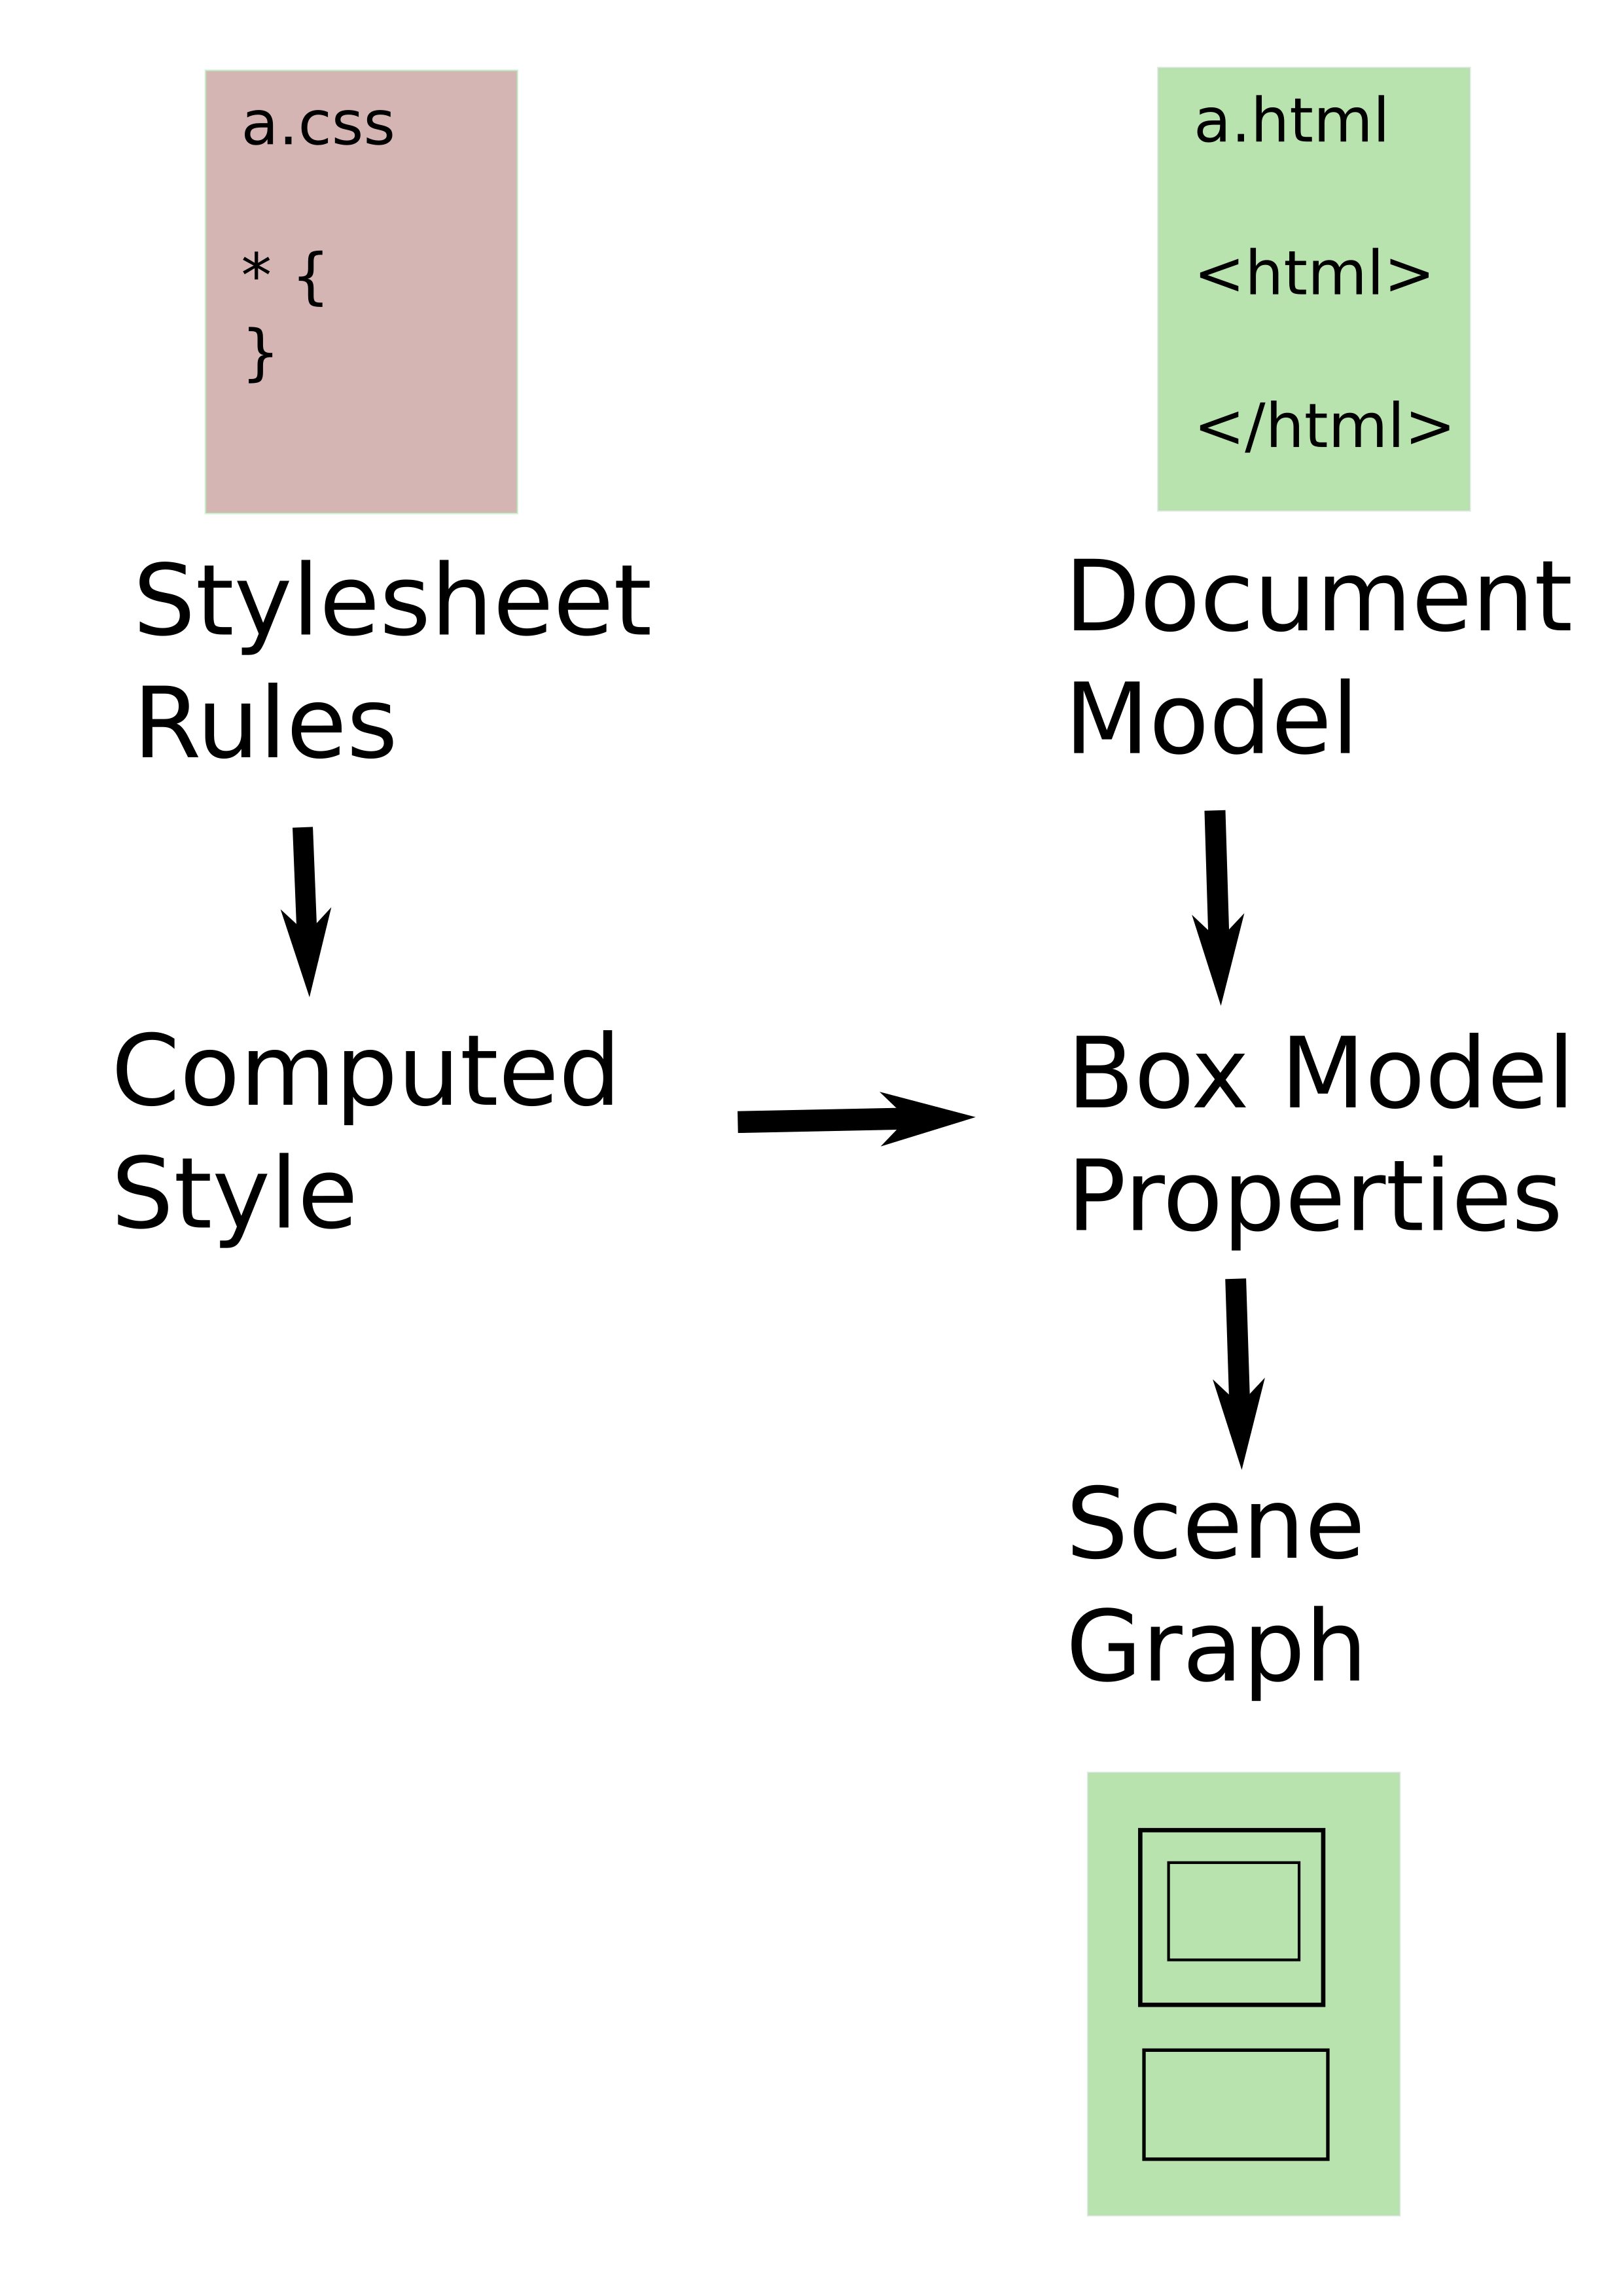
\includegraphics[width=\linewidth]{diagram.png}
  \caption{The process of rendering a CSS file and an HTML file
    to a scene graph. The CSS file is parsed into stylesheet rules,
    which are cascaded to produce a computed style for each element.
    From the computed style and the document model,
    box model properties can be computed for each element,
    which are then used to lay out the document as a collection
    of boxes in a scene graph.
    \name recieves the document model and final scene graph as input,
    and computes the stylesheet rules by inverting the usual rendering process.}
\end{figure}

The process of rendering an HTML page
  given the constraints described in a CSS file is partially defined
  by the CSS specification and partly by the common behavior of browsers.
The rendering process proceeds from the parsed HTML page,
  any associated CSS files, and the rendering context
  (type of device, screen resolution, screen size, and so on).
First, for each element, the set of matching rules is found.
Any conflicts between the matching rules are resolved
  by ordering them by the selectors used, the source of the rule,
  and the position of the rule in its CSS file.
This yields, for each element in the HTML file,
  a \textit{computed style} which contains a value
  for each applicable CSS property.
The computed styles are then used to compute various
  \textit{box model properties} of the element,
  such as its padding, the gap between it and the previous element, and so on.
Finally, these box model properties are used
  to compute a set of \textit{scene graph boxes} for the element,
  including borders, background colors, and invisible container boxes.
Each of these abstract steps is built up from several concrete steps;
  for example, computing the box model properties requires
  several top-down and bottom-up traversals of the document.
However, \name often does not model these lower-level steps
  since the presence of a complete SMT solver
  renders them unnecessary.

\section{Overview}

To synthesize CSS files
  from concrete layouts of concrete documents,
  \name uses Z3
  to render the concrete documents with a symbolic CSS file,
  require it to produce the required layout,
  and ask the solver to produce a concrete CSS file
  that fulfills this requirement.
\name receives as input a collection of trees representing HTML documents,
  a bound on the number of CSS rules to generate,
  the width of the browser window for the render,
  and a set of constraints on the final render for each HTML document.
These constraints may be arbitrary Z3 functions,
  but usually exactly specify the position and size of boxes
  (lines of text, paragraphs, images) in the final output.
For example, \name can be asked to generate a three-rule CSS file
  for the HTML document
\begin{pseudocode}
  \htmlpretty{<html><body>\><div_1></div_1>\><div_2></div_2>\></body></html>}
\end{pseudocode}
  such that, when rendered in an 800-pixel-wide window,
  the \textsf{body} is $600\times400$ pixels and located at $(100, 0)$,%
  \footnote{As an $(x, y)$ coordinate from the top-left corner,
    with the first axis pointing right and the second pointing down.}
  the $\mathsf{div_1}$ is $400\times100$ pixels and located at $(200, 66)$,
  and the $\mathsf{div_2}$ is also $400\times100$ pixels and located at $(200, 233)$.
\name may then generate the CSS file
\begin{pseudocode}
* \;\{ \\
\> \T{margin}:\: \T{auto} \\
\} \\
\T{body} \;\{ \\
\> \T{padding}:\: 66\T{px}\;0\;1\T{px}; \\
\> \T{width}:\: 600\T{px};\\
\> \T{height}:\: \T{334}\T{px} \\
\} \\
\T{div} \;\{ \\
\> \T{height}:\: 100\T{px};\\
\> \T{width}:\: 400\T{px};\\
\> \T{margin-bottom}:\: 66\T{px} \\
\}
\end{pseudocode}
\name can also optimize CSS files,
  attempting to minimize the length of the file in lines.
For example, the style sheet file above is not optimal:
  the \T{margin} declaration in the $*$ block
  could be copied to the \T{body} and \T{div} rules, saving a line;
  then the resulting two margin declarations
  in the \T{div} rule can be merged to save another line.
\name can do such optimization automatically.

\section{CSS Semantics}

\name models a subset of the rendering process
  which takes place within a browser.
As in a browser, \name models a CSS file as a collection of rules,
  each of which includes a collection of properties and a selector.
For each document object,
  the rules are filtered to those whose selectors match this object
  and cascaded to yield the computed style of that element.
From this computed styles,
  the scene graph box of the document object is computed,
  including its position on the screen.
The screen position, width, and height are then extracted
  to produce a scene graph.
Constraints are placed by the user
  upon the scene graph and the document objects,
  describing the initial document and its final render,
This scene graph then corresponds directly to the final render.
Each of these steps are defined as Z3 constraints
  and so can be inverted,
  computing the style sheet from the final scene graph.
This subsection describes how each of these steps
  are defined as Z3 formulas.

\subsection{Data types}
\name models the internals of a browser
  with four core data types:
\begin{itemize}
\item Document objects, which are block or inline elements.
  each has pointers to a parent, first and last child, and previous sibling.
  Each document object also has a computed style and a scene graph box.
\item Computed styles, which contain a value for every CSS property.
  For cascading, each also contains a score for each property.
\item Stylesheet rules, each of which contains a selector
  and a value for each CSS property (or a flag if that property is not specified).
\item Scene graph boxes, which represent the final layout of a document object.
\end{itemize}
\name instantiates one document object
  for each element of each input document,
  including instantiating a computed style and a scene graph box.
The pointers to parent, sibling, and child elements are given concretely
  as dictated by the tree structure of the input document.
\name also instantiates a number of stylesheet rules.
A set of cascading constraints then
  connects each element's computed style to these stylesheet rules,
  and a set of layout constraints
  connects each element's computed style to its scene graph box.
The user gives constraints on the scene graph box
  to describe the rendering context and
  the correct layout of the document.

\subsection{Cascading}
Cascading determines
  what value a property should take in a computed style for an element
  when multiple stylesheet rules match that element.
All matching rules which specify a value for the property are ranked,
  and value of the highest-ranked rule is used.
\name represents this ranking with a score
  that is computed from the rule's selector.
To implement cascading,
  the computed style stores, along with the value each property,
  the score of the highest-ranked computed style
  which matches the element
  and specifies the style.
Then the score is constrained to be greater than or equal
  to the score of any matching rule.
Finally, one rule must apply,
  have the property enabled,
  have a score equal to the score in the computed style,
  and have a value equal to the value in the computed style.
Symbolically, this is the conjuction of one constraint
  for each element $e$ and its computed style $s$,
  each property $p$,
  and each stylesheet rule $r$:
\[
r.\mathsf{enabled}(p) \land
\mathsf{applies}(r, e) \implies
s.\mathsf{score}(p) \ge \mathsf{score}(r).
\]
Furthermore, each property must take its value
  from the highest-ranked rule:
\[
\bigvee_{r} \quad
\begin{align*}
& r.\mathsf{enabled}(p) \land \mathsf{applies}(r, e) \land \\
& \mathsf{score}(r) = s.\mathsf{score}(p) \land r.\mathsf{value}(p) = s.\mathsf{value}(p).
\end{align*}
\]
The \textsf{score} function and the \textsf{applies} predicate
  are implemented as functions in Z3,
  which look at the rule's selector
  to compute its score and determine if it applies to an element.
This allows Z3 to reason about
  whether certain selectors apply to an element or not,
  and thus allows Z3 to choose the selectors.

\subsection{Layout of block elements}
Once cascading has determined the computed style for each element,
  that style can be used to constrain
  the position, padding, and margins of the element.
Some of these constraints are simple;
  for example, is the computed style
  gives the padding of an element in pixels,
  that element's padding is precisely the given value.
However, some properties are more complex.
For example, CSS allows independently specifying
  the left and right margins, left and right padding,
  and width of an element,
  and specifies rules to be followed
  if the total padding, margin, and width exceed that of the parent,
  which differ depending on whether one, some, or all
  of the width and the left and right margins are set to ``auto''.
Each of these rules is rendered as a Z3 formula;
  for example, Section~10.3.3,
  which describes how ``auto'' margins and widths are resolved,
  is encoded as the following formula:
\begin{pseudocode}
\K{let} m_l \ceq (s.\T{margin}_l = \T{auto} ? 0 : s.\T{margin}_l) \\
\K{let} m_r \ceq (s.\T{margin}_r = \T{auto} ? 0 : s.\T{margin}_r) \\
\K{let} w \ceq e.\T{padding}_l + e.\T{padding}_r + e.\T{width} + m_l + m_r \\

s.\T{width} \ne \T{auto} \land w  > e.\T{parent}.\T{width} \implies \\
\> (s.\T{margin}_l = \T{auto} \implies e.\T{margin}_l = 0) \\
\> (s.\T{margin}_r = \T{auto} \implies e.\T{margin}_r = 0) \\
(s.\T{width} = \T{auto} \land s.\T{margin}_l = \T{auto})
\implies e.\T{margin}_l = 0 \\
(s.\T{width} = \T{auto} \land s.\T{margin}_r = \T{auto})
\implies e.\T{margin}_r = 0 \\
(s.\T{margin}_l = \T{auto} \land s.\T{margin}_r = \T{auto})
\implies e.\T{margin}_l = e.\T{margin}_r
\end{pseudocode}
In total, the fragment of CSS that \name supports
  is encoded as 14 non-trivial constraints.

\subsection{Layout of inline elements}
Inline elements are laid out differently from block elements.
Unlike block elements,
  CSS allows multiple inline elements to sit side-by-side,
  and allows inline elements to wrap across lines.
Inline elements also use different rules for margins and padding,
  and interact non-trivially with the block elements that contain them.
Line wrapping presents a particular difficulty to \name,
  since line wrapping is language- and font-dependent;
  that is, it is not something we can efficiently model in Z3.
A true browser would break lines based on the words in the line,
  browser-specific line-breaking heuristics,
  and a language model that described where line breaks are appropriate,
  along with any manually-added non-breaking spaces and soft hyphens.
Instead of modeling this complexity,
  \name assumes that all line wrapping is done correctly
  by whatever tool the designer used to generate constraints,
  and requires that the width and height of each line,
  and the text width of each paragraph, be given concretely.

\subsection{Selectors}

\name models only a small subset of the selectors in CSS:\@
  a single tag-name pattern such as \textsf{H1}
  and the universal pattern $*$.
Each stylesheet rule has an associated selector,
  and \name does not constrain the selectors in any way,
  allow Z3 to generate any selectors
  that successfully generate the required CSS file.
Two functions are defined on selectors:
  a predicate that determines whether a selector matches an element,
  and a function to compute a selector's score for cascading.
Determining whether a selector $s$ matches an element $e$ is simple:
\begin{pseudocode}
s = * \lor (s = \T{Tagname}(t) \land e.\T{tagname} = t).
\end{pseudocode}
Computing the score is similarly easy;
  scores are represented by six-tuples,
  with two entries describing the source,
  one counting the number of id patterns in the selector,
  one counting the number of class patterns,
  one counting the number of tag name patterns,
  and one describing the position of the rule in the style sheet file.
Since \name only supports single tag-name selectors
  and the universal selector,
  only two of the fields
  (number of tag name patterns and position in the file)
  are used.

\subsection{Optimization of Synthesized CSS}

Many CSS files produce equivalent renders and Z3, without guidance,
  produces baroque and overly-complex stylesheets.
To prevent this, \name asks Z3 to optimize for short stylesheets;
  in particular, stylesheets with few lines.
Each CSS rule costs two lines if any of its properties are enabled,
  and each enabled rule costs one additional line.
Shorthand properties like \texttt{margin} and \texttt{padding}
  allow saving three lines if all four directions are enabled.
These three rules are the only ones governing the cost model;
  each is encoded as a soft assertion, and Z3's \texttt{opt} branch
  is used to minimize the total cost of the violated soft assertions.
This simple cost model causes Z3 to generate relatively short CSS files,
  which avoid unnecessary operations.
In the future, we hope to extend the cost model
  to count byte-level, as opposed to line-level, length.
Optimization for byte size will translate into ready gains
  by minimizing the size of the CSS file
  that must be sent over the internet to the user.

\section{Evaluation}

We evaluate \name by asking it to synthesize two pages
  from the first author's website.
A variety of font properties are extracted from the original CSS file,
  and added as a hardcoded block to the top of \name's output,
  since \name does not track font properties.
To collect the constraints, we used a Javascript program
  run a browser rendering the pages
  to gather positioning information for each box.
Both pages contained several paragraphs of text;
  one mixed these paragraphs with blocks of code,
  and the other used small amounts of inline markup
  long with ordinary block layout.
Both pages contained some number of ``invisible'' elements---%
  elements that grouped paragraphs of text,
  but did not themselves leave visible traces.
We conducted three experiments synthesizing these two pages:
  a run without optimization,
  and with constraints about the positioning of each element
  (including the invisible ones);
  a run without optimization,
  and with information only about the positioning of text
  (no constraints governing the behavior of invisible elements);
  and with optimization for size and constraints
  on each element's position.
In each case, \name was limited to four CSS rules;
  fewer were not sufficient, and more were unnecessary.
Each experiment used Z3 version 4.3.2, and for each,
  the resulting CSS file was viewed in Firefox 36
  and Chromium 40.0.2214.115.

Each experiment yielded a CSS file that,
  when rendered by both Firefox and Chromium,
  perfectly reproduced the original rendering of the web page.
Without optimization for size, the CSS files were 37 lines long,
  compared to 26 lines for the website's original, human-authored stylesheet.
With optimization for size enabled, the CSS files were 15 lines long,
  significantly shorter than the human-authored stylesheet.
The first experiment, with no optimization and all constraints,
  had a synthesis time of $26.4 \pm 0.5$ seconds;
  the second, with no optimization but only constraints on the text position,
  took $174 \pm 10$ seconds;
  and the third, with optimization and all constraints,
  took $155 \pm 8$ seconds.

\section{Related Work}

Thibaud Hottlier investigated the possibility
  of generating efficient layout engines
  given a language of constraints for that engine to solve~\cite{thibaud-thesis},
  and developed a method of \emph{programming by manipulation}
  to allow users to design the language of constraints
  by manipulating example documents~\cite{thibaud-uist}.
Unlike \name, this method does not synthesize constraints
  for individual documents;
  instead, it only synthesizes a layout engine
  which can lay out constraints written by users.
Several papers have focused on CSS layout in the browser,
  with a focus on making layout parallelizable~\cite{fast-parallel-layout,fast-browser}.
Bricolage~\cite{bricolage} used structured prediction
  to transfer web design styles between web pages,
  learning from human examples.
Webzeitgeist~\cite{webzeitgeist} is a repository
  of over 100,000 web page designs;
  combined with Bricolage,
  it could be used to create designs for new web pages
  by pasting together aspects of web page designs from existing pages.
However, this approach could not be used to create novel web designs,
  nor does it allow optimizing the resulting designs
  for short style sheet files.
SeeSS~\cite{seess} helps designers visualize the effects of CSS changes
  across all of the pages in a website,
  avoiding the problem of a change improving the layout of one page
  while introducing layout problems to another page.
SeeSS highlights the importance and difficulty of generalization
  for style sheet files, a difficulty \name resolves
  by synthesizing style sheets that simultaneously lay out
  multiple web pages.

\section{Conclusion}

\name automatically generates CSS files
  given a description of how a concrete web page should render.
In doing so, it automates a task
  human designers traditionally have to do by hand,
  and furthermore allows optimization
  that is difficult for humans.
\name demonstrates that the general task of constraint synthesis
  is tractable, and can improve the experience
  of writing constraint-based layouts.

\begin{thebibliography}{9}

\bibitem{thibaud-thesis}
  Thibaud Hottelier,
  Programming Layout by Manipulation.
  Ph.D. thesis, University of California at Berkeley.
  \href{http://www.eecs.berkeley.edu/Pubs/TechRpts/2014/EECS-2014-158.html}{Technical Report EECS-2014-158}.

\bibitem{thibaud-uist}
  T. Hottelier, R. Bod\'ik, and K. Ryokai.
  Programming by manipulation for layout,
  UIST 2014. pp. 231--241.

\bibitem{fast-parallel-layout}
  L. A. Meyerovich and R. Bod\'ik.
  Fast and parallel webpage layout,
  WWW 2010, pages 711–720. 

\bibitem{fast-browser}
  C. Jones, R. Liu, L. Meyerovich, K. Asanovic, and R. Bodik.
  Parallelizing the web browser.
  Usenix HotPar 2009. 
  
\bibitem{bricolage}
   R. Kumar, J. O. Talton, S. Ahmad, S. R. Klemmer.
   Bricolage: Example-Based Retargeting for Web Design,
   CHI 2011.

\bibitem{webzeitgeist}
  R. Kumar, A. Satyanarayan, C. Torres, M. Lim, S. Ahmad, S. R. Klemmer, J. O. Talton.
  Webzeitgeist: Design Mining the Web,
  CHI 2013. 
  
\bibitem{seess}
  H. Liang, K. Kuo, P. Lee, Y. Chan, Y. Lin, M. Chen.
  SeeSS: seeing what I broke---visualizing change impact of Cascading Style Sheets (CSS),
  UIST 2013.


\end{thebibliography}

\end{document}
